%==============================================================================
\chapter{Theory}
\label{sec:theory}
%==============================================================================

In this chapter, the theoretical background of this thesis will be discussed
in detail. This covers both physics as well as the techniques used for data
analysis. In the physics part, we will concentrate on neutrinos and their
properties and interactions, with special emphasis on neutrino oscillations.
The analysis part will describe the Fisher Information Matrix as a tool to
efficiently characterise a multi-dimensional likelihood landscape.

%==============================================================================
\section{Neutrinos}
\label{sec:nus}
%==============================================================================


\subsection{Neutrinos in the Standard Model}
\label{sec:NusInSM}

In the Standard Model of Particle Physics, or just Standard Model, the current
theories of the electroweak and strong interactions are combined
\cite{SMGlashow, SMWeinberg, SMSalam, SMtHooft}, for an overview see e.g.\
\cite{SMtextbook}. It is a quantum field theory of the fundamental interactions
and particles relevant on the scales that are accessible for particle physics
experiments.

\begin{figure}
\centering
  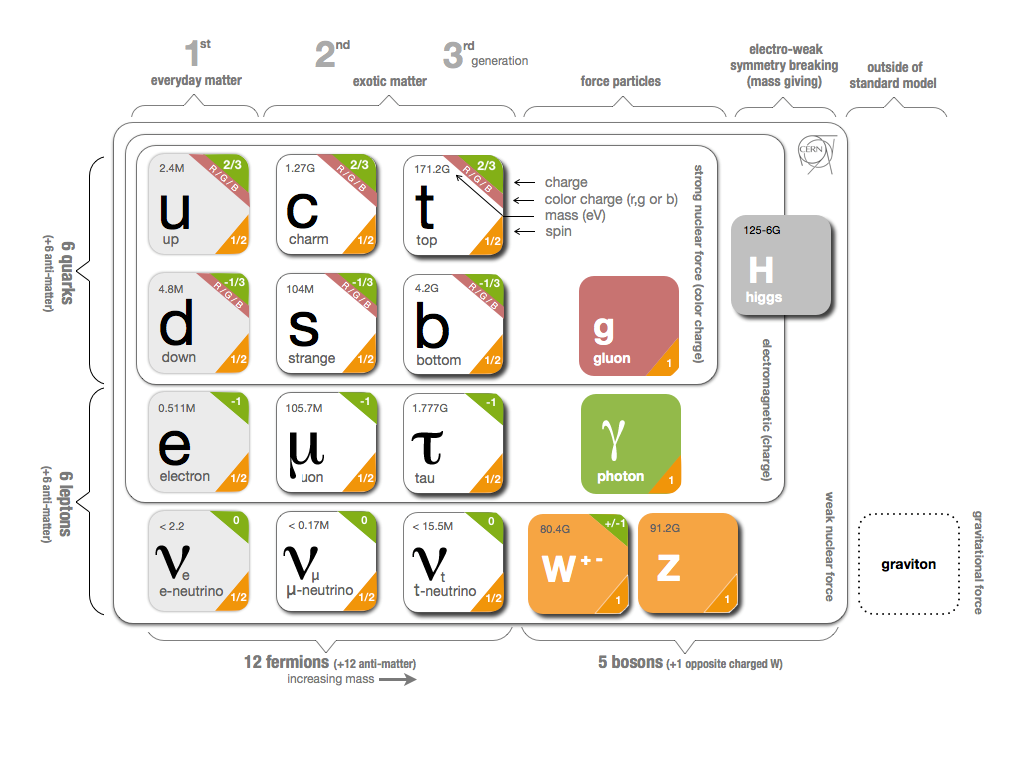
\includegraphics[width=0.8\textwidth]{Standard_model_infographic}
\caption{The fundamental particles in the Standard Model \cite{SMchart}.}
\label{fig:SMchart}
\end{figure}

The particles, listed in Fig.~\ref{fig:SMchart} can be divided in two classes:
fermions with an intrinsic spin of 1/2 make up everything that is usually called
``matter'', and exchange bosons with integer (1 in most cases) spin that convey
the interactions and couple to the respective charge. Formally, the bosons are
the generators of the gauge symmetry group of the particular interaction.

This means that the strong force, which obeys a \emph{SU(3)} symmetry, has eight
generators that are represented by eight gluons $g$. The gluons couple to the
strong charge which is usually referred to as ``colour''. Since it has the
largest coupling constant, the strong interaction is dominant whenever a
colour charge is present. However colour is ``confined'', i.e. free particles
must not have a net colour. This means that any coloured particles have to be
bound inside a compound object at all times. Also, the range of the strong
interaction is limited to about the size of a nucleus since the gluons are
coloured themselves and hence self-coupling.

About two orders of magnitude weaker is the electromagnetic interaction.
According to its \emph{U(1)} symmetry, it has only one exchange boson, the
photon $\gamma$, coupling to the electrical charge. It is massless and
electrically neutral, hence the electromagnetic interaction is not restricted
in range. This and the fact that there is no confinement on the electrical
charge mean that on macroscopic scales electromagnetic phenomena are dominant.

At low energies, the effective coupling constant of the weak interaction is
another three orders below the electromagnetic one. From its \emph{SU(2)}
symmetry originate three exchange bosons, $W^\pm$ and $Z^0$ with masses of
about 90\,MeV limiting its range to the subatomic scale. However with increasing
energy, the mass of the gauge bosons becomes more and more negligible and the
effective coupling rises. Above the electroweak unification at about 100\,GeV,
the weak and electromagnetic interactions can be described by one unified
theory, whose existence is also hinted to by the fact that the weak gauge
bosons are electrically charged.

Their masses arise from another spontaneously
broken local \emph{SU(2)}$\times$\emph{U(1)} symmetry of the so-called
Higgs\footnote{After Peter Higgs, who, together with others, laid the
foundations of this theory in the 1960's \cite{Higgs, BroutEnglert}.} field.
After breaking, the generators of the \emph{SU(2)} part mix with the weak
bosons, giving them mass, while the generator of the remaining \emph{U(1)} can
be observed as the only scalar gauge boson, the Higgs boson. The Higgs boson
was the last fundamental particle of the standard model to be detected, its
discovery was claimed by the ATLAS and CMS collaborations in 2012
\cite{AtlasHiggs, CMSHiggs}.

The other group of fundamental particles are the fermions (and their
corresponding antiparticles). They can be divided again into two subclasses: the
six quarks $u,\ d,\ c,\ s,\ t$, and $b$, which obey all forces and---being
coloured---are confined, so that no free quarks can be found in nature. Bound
quarks are making up baryons, like protons and neutrons, consisting of three
quarks, and unstable mesons, which consist of a quark and an antiquark, like
pions. Baryons and mesons, together called hadrons, are the only free particles
participating in the strong interaction, since they contain coloured quarks,
although not being coloured themselves.

The second subclass are the leptons, the three charged leptons $e$, $\mu$, and
$\tau$, as well as the corresponding (neutral) neutrinos \nue, \numu, and
\nutau. The charged leptons interact predominantly electromagnetically, most
prominently electrons are bound to nuclei via electrical attraction. However
the decay of $\mu$ and $\tau$ is---like every flavour-changing process---a weak
interaction. The electron as the lightest charged lepton has to be stable due
to conservation of energy and charge.

Since neutrinos are neither coloured nor electrically charged, they only
interact weakly. This means that they are very hard to detect directly. In
fact, their existence had already been suggested in 1930 by Wolfgang Pauli as a
solution for the problem of missing energy in radioactive $\beta$ decays
\cite{PauliBeta}. However the first direct detection of (electron) neutrinos,
\nue, from a nuclear reactor was achieved only in 1956 in the so-called
Cowan-Reines experiment \cite{CowanReines}. The existence of a second neutrino,
the muon neutrino \numu, was established few years later in 1962 from the study
of charged pion decays \cite{NuMuDiscovery}. The third neutrino, the \nutau,
was finally discovered directly by the DONUT experiment in 2001 in the decay of
$D_S$ mesons into \nutaubar and $\tau$, which again decay into \nutau and other
leptons \cite{DONUT}.

In addition to having neither colour nor electrical charge, the standard model
also predicts that neutrinos are massless. Thus the observation of neutrino
oscillations by the Super-Kamiokande experiment in 1998\footnote{Hints of
neutrino oscillations had already been observed in the 1960's
\cite{DaviesNuOsc}, but were widely refused by the scientific community.}
\cite{SuperKosc} gained much attention, this being the first detection of
physics beyond the standard model.

The term ``neutrino oscillations'' describes the phenomenon that neutrinos,
when propagating over macroscopic distances, can change their flavour
eigenstate on the way between production detection. The details of this effect
will be described in Sec.~\ref{sec:osc}. However it can only occur when there
are different mass eigenstates available for the neutrinos, meaning that only
one of them---if any---can have mass zero, while the others must correspond to
finite mass.

Since their first observation, neutrino oscillations have been a field of
intensive research. After establishing all oscillation channels, nowadays the
precise measurement of the parameters that characterise the oscillation is in
the focus. The planned PINGU experiment (see Sec.~\ref{sec:PINGU}), whose
simulation is the main topic of this thesis, is aimed to reach unprecedented
accuracy in measuring the parameters \thet{23} and \dm{31}.


\subsection{Neutrino Sources}
\label{sec:NuSources}

As discussed above, neutrinos do not participate in the strong and
electromagnetic interaction, leaving only weak processes for them to be created
or detected. On the other hand, neutrinos are produced in nearly every weak
interaction, making them a very common particle that can stem from a variety of
different sources in very different energy ranges.

\subsubsection{Natural Radioactivity}
On Earth, the most common source is the $\beta$ decay of natural radionuclides.
Depending on the type of the decay ($\beta^+$ or $\beta^-$), an electron
(anti-) neutrino is emitted along with the charged lepton. The general
equations read:
\begin{eqnarray}
 \beta^+: & ^A_Z\mathrm{X} & \to\quad  ^A_{Z-1}\mathrm{Y} + e^+ + \nue \\
 \beta^-: & ^A_Z\mathrm{X} & \to\quad  ^A_{Z+1}\mathrm{Y} + e^- + \nuebar
\end{eqnarray}
Examples for typical $\beta$ emitters are $^{40}$K (both $\beta^+$ and
$\beta^-$) and intermediate products from the decay chains of $^{232}$Th or
$^{238}$U ($\beta^-$), the neutrino energies are usually on the scale of few
MeV.

In fact, the $\beta$ decay was the original reason to propose the existence of
the then un-detectable neutrino. Since only the daughter nucleus and the
charged lepton were visible as decay products, the process seemed to be a
two-body decay. This means that the energies of the decay products are exactly
determined from kinematics and hence the emitted electrons or positrons would
be monoenergetic. Observations showed, however, a broad spectrum in energy
instead of a single line. Without violating the conservation of energy, this
can only be achieved if a third particle is produced in the process, which is
electrically neutral but can carry away energy and momentum. 

On the subatomic level, in a $\beta^+$ decay one proton inside a nucleus emits a
virtual $W^+$ boson, turning an $u$ into a $d$ quark, and becomes a neutron.
During a $\beta^-$ decay, the opposite happens via the emission of a $W^-$, as
shown in Fig.~\ref{fig:beta_minus}. The $W$ boson subsequently decays into a
charged lepton and a neutrino.

\begin{figure}
 \centering
 \begin{fmffile}{beta_minus}
 \begin{fmfgraph*}(80,50) \fmfpen{thin}
 \fmfstraight
  \fmfleft{i0,i1,i2,i3,i41,i42,i5,i51,i6}
  \fmfright{o0,o1,o2,o3,o41,o42,o5,051,o6}
  \fmf{fermion}{i0,o0}
  \fmflabel{$u$}{i0}
  \fmflabel{$u$}{o0}
  \fmf{fermion}{i1,o1}
  \fmflabel{$d$}{i1}
  \fmflabel{$d$}{o1}
  \fmf{fermion}{i2,v1,o2}
  \fmflabel{$d$}{i2}
  \fmflabel{$u$}{o2}
  \fmffreeze
  \fmf{fermion}{o5,v2,o6}
  \fmflabel{$e^-$}{o6}
  \fmflabel{\nuebar}{o5}
  \fmf{dashes,lab=$W^-$,l.side=left,tension=1.5}{v1,v2}
 \end{fmfgraph*}
 \end{fmffile}
 \write18{mpost beta_minus}
\caption{Feynman diagram of a $\beta^-$ decay}
\label{fig:beta_minus}
\end{figure}

% TODO: say something about 0n2b decay?


\subsubsection{Nuclear Reactors}

In nuclear reactors, the controlled fission of heavy elements is used for the
generation of electrical power. The intermediate products of these nuclear
fissions are unstable isotopes that usually have a large surplus of neutrons
compared to a stable configuration. These unstable nuclides undergo a series of
$\beta^-$ decays until they they reach a stable ratio of proton and neutron
numbers.

Since in each of those $\beta$ decays neutrinos are emitted, a nuclear reactor
provides a strong and steady flux of \nuebar, which can be monitored via the
thermal power of the reactor. This makes reactor neutrinos a popular target for
experiments, especially for the study of neutrino oscillations. The main
challenge in such experiments is the accurate modelling of the neutrino energy
spectrum, which is the sum of the spectra of all of the different $\beta$
decays in the decay chain. Even though there are very elaborate flux models
available, there might still be components unaccounted for, resulting in
unexpected features in the measured neutrino flux \cite{RENO_5MeV}.


\subsubsection{Neutrino Beams}

Another artificial source of neutrinos, but somewhat higher in energy
(typically at a few GeV) are neutrino beams. Since the neutral neutrinos cannot
be accelerated directly, usually a high-energy, high-intensity proton beam is
aimed at a target in which it produces mesons, mostly pions and kaons, in whose
subsequent decay neutrinos are produced \cite{NuBeams}:
\begin{eqnarray}
 \pi^+ & \to & \mu^+ + \numu \\
 \pi^- & \to & \mu^- + \numubar
\end{eqnarray}

Such beams are the source of neutrinos that can be controlled best in terms of
energy and intensity, making them a preferred choice for precision experiments
such as measurements of neutrino cross-sections. However they are very expensive
to build and operate in contrast to natural sources or nuclear reactors, the
latter usually being operated by commercial power suppliers.


\subsubsection{Solar Neutrinos}


\subsubsection{Atmospheric Neutrinos}
\label{sec:AtmNus}


\subsubsection{Astrophysical Neutrinos}

\subsection{Detection of Neutrinos}